\section{Pruebas y evaluación}\label{sec:pruebas_y_evaluacion}

\subsection*{Desarrollo del conjunto de datos de prueba}

Una parte fundamental de este TFG fue construir un conjunto de pruebas que permitiera dar soporte tanto al
desarrollo como a la validación del proyecto.

En una primera aproximación se realizó una investigación sobre distintas bases de datos que ofrecen
conjuntos de datos abiertos, aquí una lista de algunas de las que investigamos:

\begin{itemize}
    \item \textbf{Data.gov}: Portal de datos abiertos del gobierno de Estados Unidos~\cite{https://www.data.gov/}.
    \item \textbf{European Union Open Data Portal}: Portal de datos abiertos de la Unión
    Europea~\cite{https://data.europa.eu/euodp/en/home}.
    \item \textbf{Kaggle Datasets}: Conjuntos de datos para competencias y proyectos de análisis de
    datos~\cite{https://www.kaggle.com/datasets}.
    \item \textbf{UCI Machine Learning Repository}: Conjuntos de datos para aprendizaje
    automático~\cite{https://archive.ics.uci.edu/ml/index.php}.
    \item \textbf{Google Dataset Search}: Motor de búsqueda de conjuntos de
    datos~\cite{https://datasetsearch.research.google.com/}.
    \item \textbf{Amazon Web Services (AWS) Public Datasets}: Conjuntos de datos públicos de
    AWS~\cite{https://registry.opendata.aws/}.
\end{itemize}

Sin embargo, no fue posible encontrar un conjunto adecuado.
Los conjuntos de datos publicados en estos portales presentan datos anonimizados.
No es posible encontrar datos como nombres, documentos de identidad, direcciónes, etc., por lo que este enfoque no fue
adecuado.

Se determinó, que el conjunto de datos de prueba debería generarse manualmente a partir de modelos descargados de
internet.

También se determinó que los conjuntos de datos deberían ser lo suficientemente grandes como para realizar pruebas que
permitieran alcanzar conclusiones relevantes en términos de precisión del sistema, pero lo suficientemente pequeños
como para que la ejecución completa de la batería no fuera excesivamente cara.

Dado que en la sección \ref{sec:implemetacion_y_programacion} Implementación y programación, se había estipulado
que el coste de la ejecución de un documento eran aproximadamente siete céntimos, se consideró que de nueve documentos
para los conjuntos de datos de prueba y de tres elementos para los conjuntos de datos de contraste, ofrecía un
balance adecuado.

En la tabla que aparece a continuación pueden verse los conjuntos de datos de prueba desarrollados.

\begin{table}[h]
    \renewcommand{\arraystretch}{1.5}
    \setlength{\tabcolsep}{10pt}
    \centering
    \begin{tabular}{>{\bfseries}p{0.15\textwidth} p{0.55\textwidth} p{0.15\textwidth}}
        \toprule
        \textbf{Conjunto} & \textbf{Contenido}                                        & \textbf{Elementos} \\
        \midrule
        \textbf{000}      & Ruido                                                     & 3                  \\
        \textbf{001}      & Contratos de arrendamiento de vivienda entre particulares & 9                  \\
        \textbf{002}      & Contratos de compra venta de vehículo entre particulares  & 9                  \\
        \bottomrule
    \end{tabular}
    \caption{Conjuntos de datos de prueba}
    \label{tab:data_sets}
\end{table}

El conjunto de datos \textbf{000} contiene ruido, es decir documentos que no corresponden a ninguno de los
otros conjuntos.

El conjunto de datos \textbf{001} contiene modelos descargados de diferentes fuentes de internet.
Se modificaron los documentos con datos generados aleatoriamente para indicar nombres, apellidos, direcciones, etc.

El conjunto de datos \textbf{002} se generó de la misma forma que el anterior.

Este proceso aseguró la privacidad y el cumplimiento de la normativa de protección de datos.



\subsubsection*{Construcción del conjunto de datos de prueba}

Para permitir modificar fácilmente los documentos de los diferentes conjuntos, estos fueron transformados a formato
\textbf{Markdown}, más sencillo de modificar, que los documentos originales en formato \textbf{Word}.

A través de \textbf{LaTeX} y diferentes plantillas para introducir variabilidad en los formatos de entrada, estos
documentos son convertidos a formato \textbf{PDF}.
En la figura~\ref{fig:chapter_4.5.dataset_construction_overview} puede verse un esquema de este comportamiento.

\begin{figure}[ht]
    \begin{center}
        
\includegraphics[width=\textwidth]{./chapter/4/images/chapter_4.5.dataset_construction_overview}
        \caption{Contrucción del conjunto de datos de prueba}
        \label{fig:chapter_4.5.dataset_construction_overview}
    \end{center}
\end{figure}


\subsection*{Pruebas automáticas}

Las pruebas automáticas son esenciales para garantizar la calidad y la robustez del software.

En este proyecto, se han implementado varios tipos de pruebas automáticas, cada una con un enfoque diferente para cubrir
todas las facetas del desarrollo y la implementación del software.

\begin{enumerate}
    \item \textbf{Pruebas unitarias}: verifican el funcionamiento de componentes individuales del sistema, como
    funciones o métodos.
    \item \textbf{Pruebas integración}: comprueban el correcto funcionamiento de diferentes componentes
    interactuando coordinadamente.
    \item \textbf{Pruebas funcionales}: evalúan el sistema desde el punto de vista del usuario final.
\end{enumerate}

En la figura~\ref{fig:chapter_4.5.test_suite_execution} puede verse el resultado de la ejecución de la batería de
pruebas.

\begin{figure}[ht]
    \begin{center}
        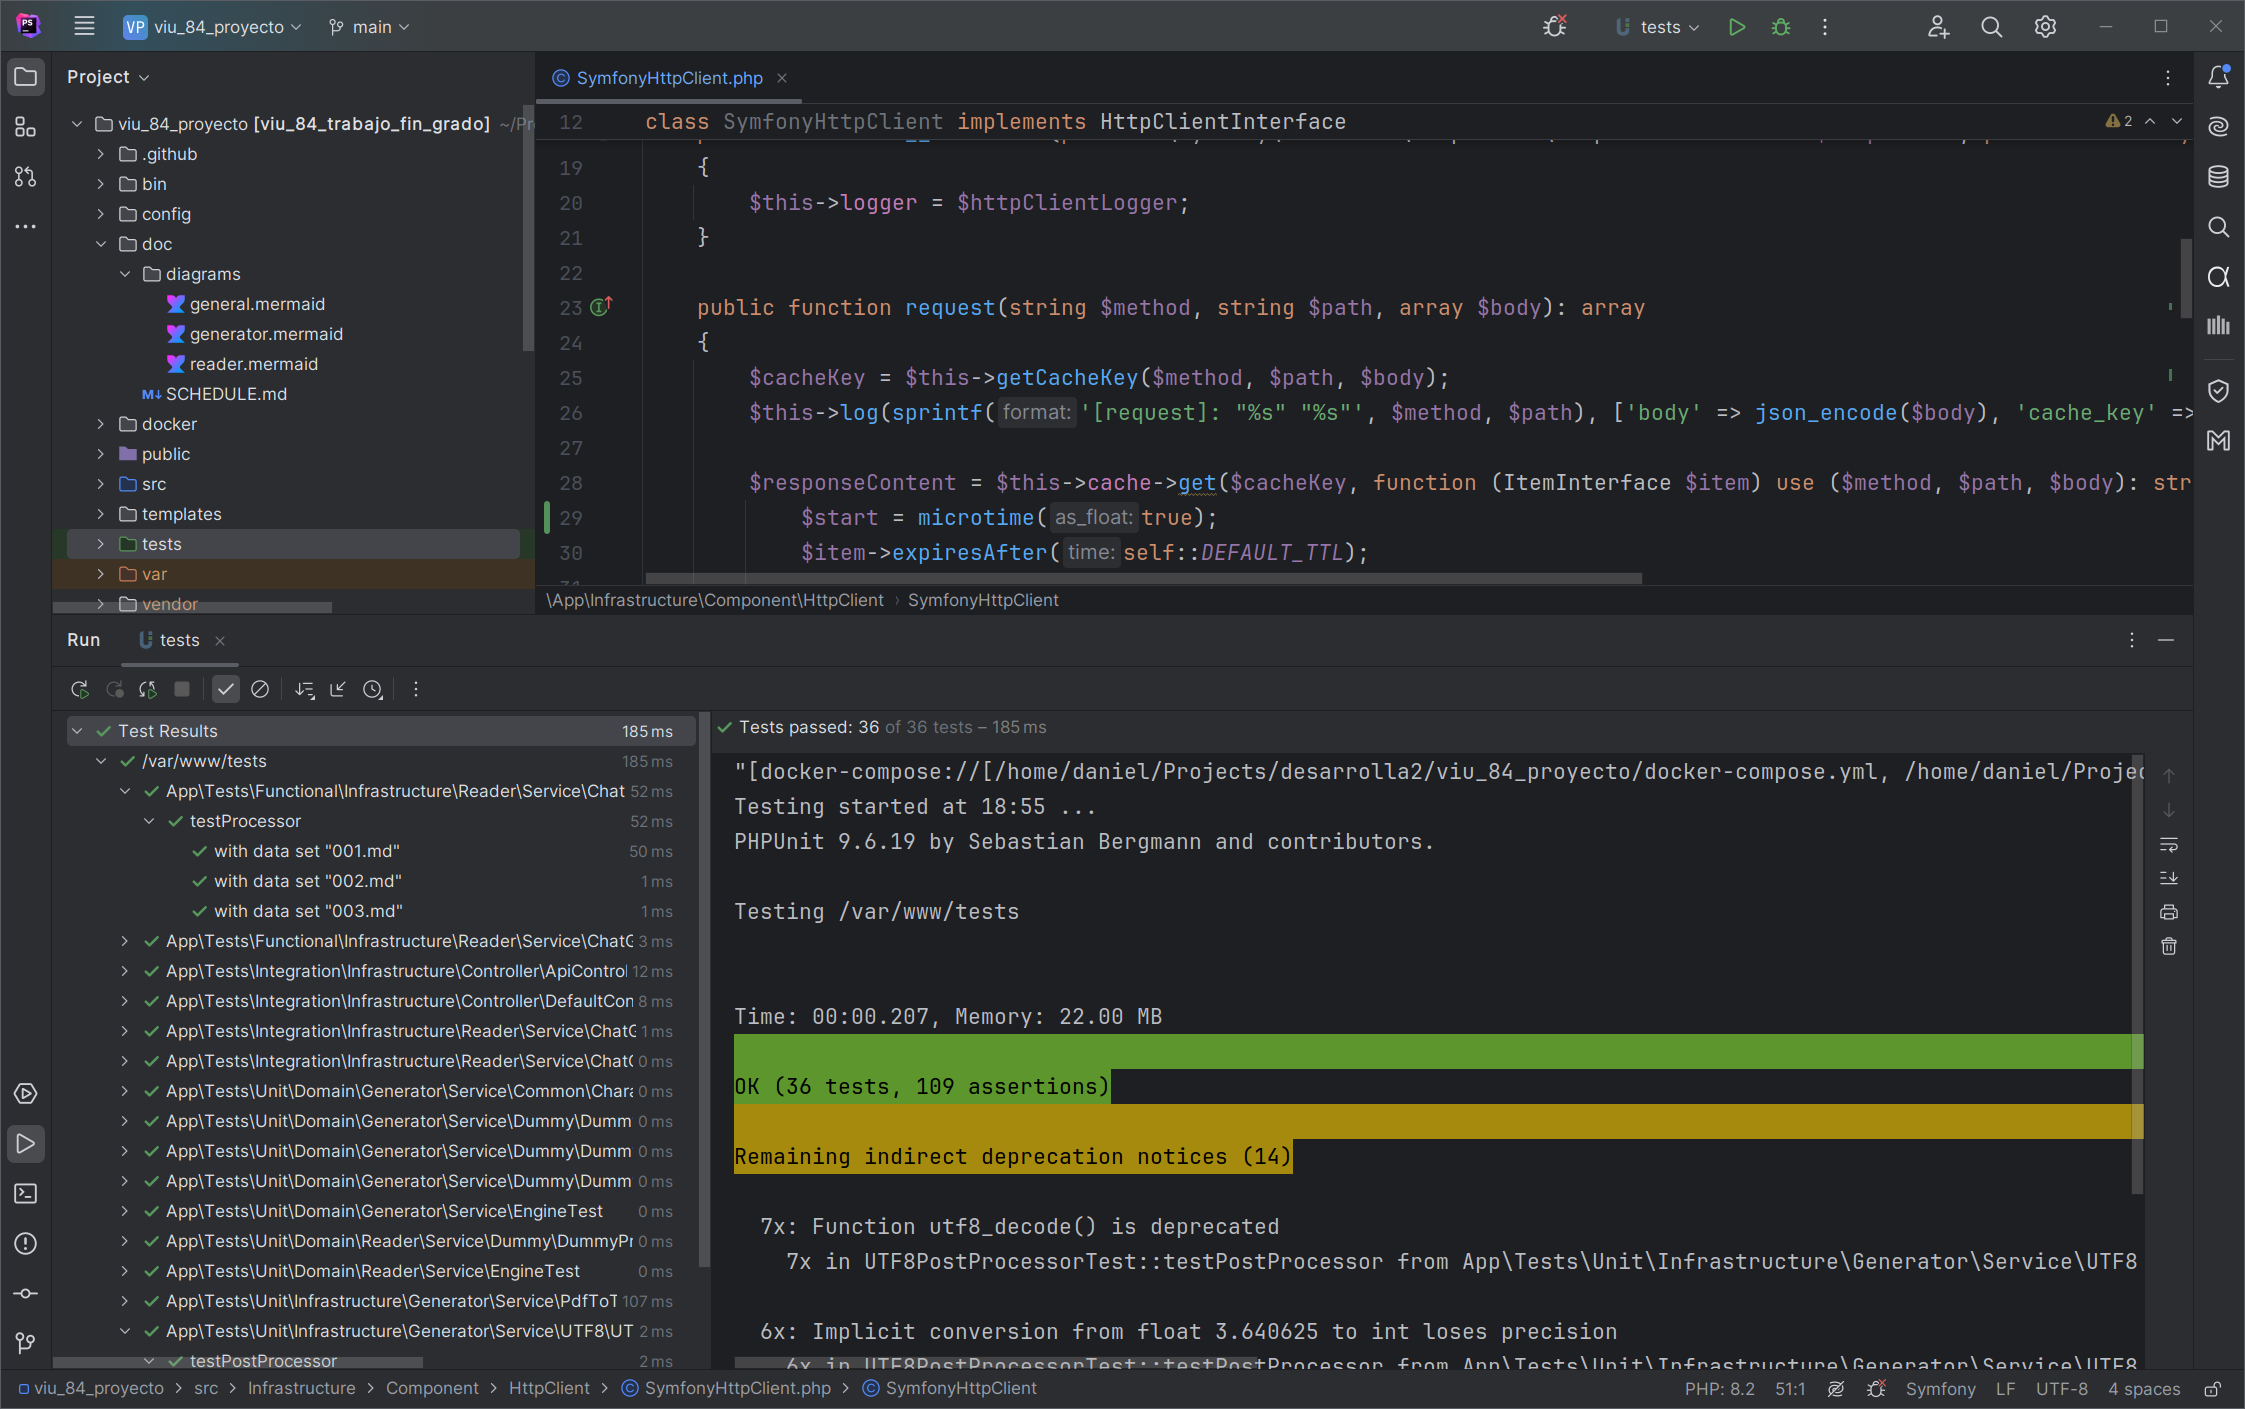
\includegraphics[width=\textwidth]{./chapter/4/images/chapter_4.5.test_suite_execution}
        \caption{Resultado de la ejecución de la batería de pruebas automáticas}
        \label{fig:chapter_4.5.test_suite_execution}
    \end{center}
\end{figure}

\subsection*{Integración continua}
La integración continua es una práctica esencial en el desarrollo de software moderno, que implica la integración
frecuente, normalmente programando la ejecución automática de los test y otras tareas en un servidor de integración
continua, cada vez que se añade un commit al repositorio.

\begin{figure}[ht]
    \begin{center}
        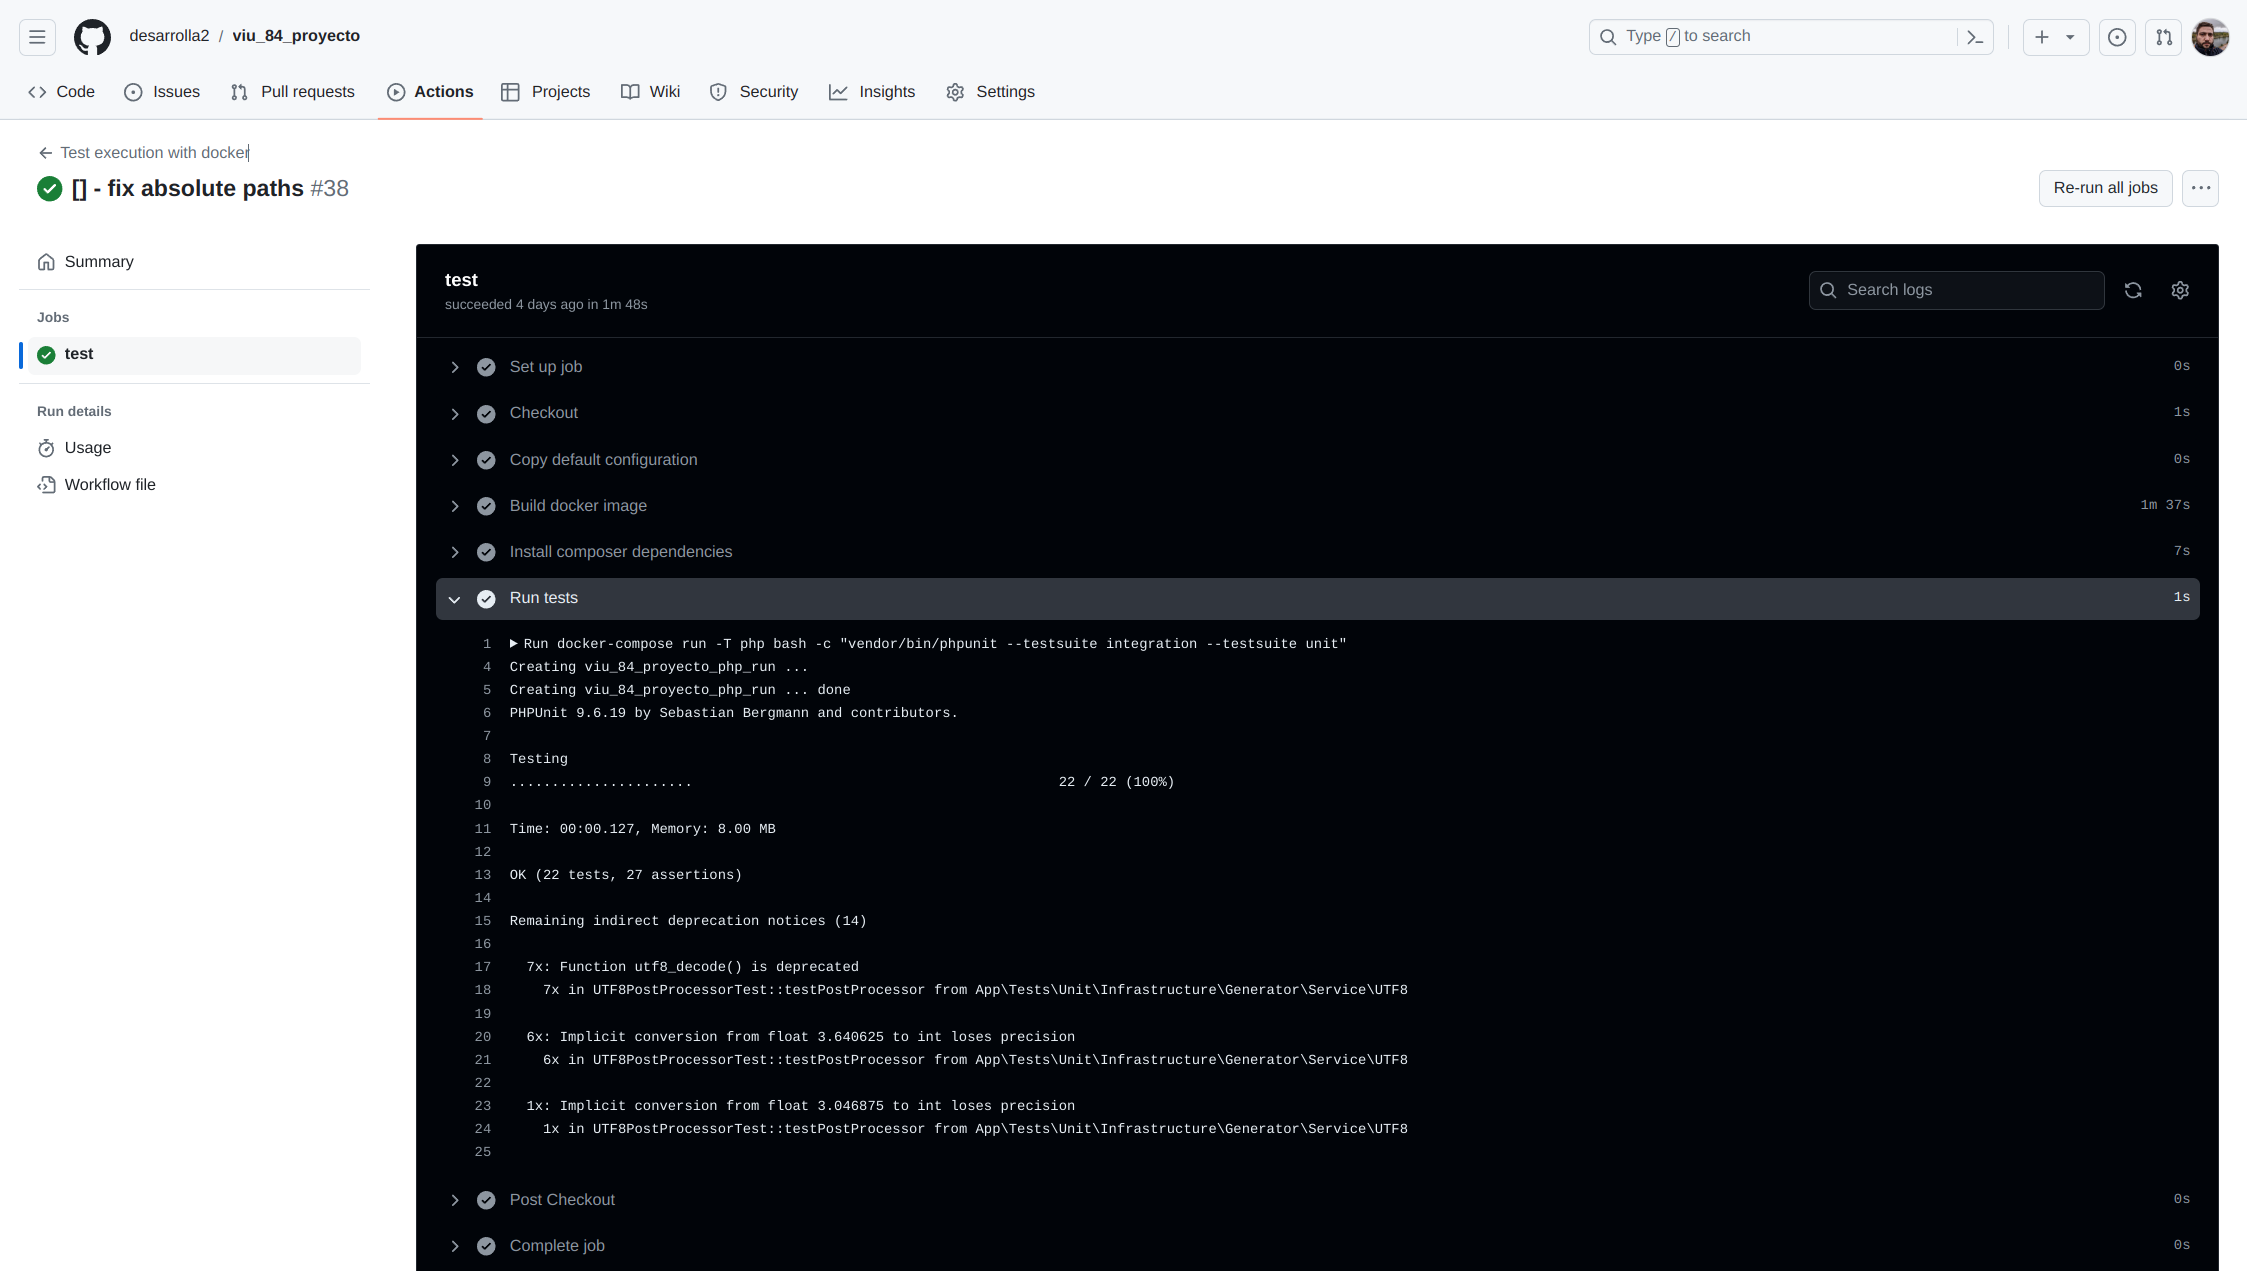
\includegraphics[width=\textwidth]{./chapter/4/images/chapter_4.5.github_actions_execution}
        \caption{Resultado de la ejecución de la batería de pruebas en el entorno de integración continua}
        \label{fig:chapter_4.5.github_actions_execution}
    \end{center}
\end{figure}

En este proyecto, hemos implementado la integración continua utilizando \textbf{GitHub Actions}, un servicio de
automatización que permite crear flujos de trabajo personalizados para compilar, probar y desplegar código directamente
desde \textbf{GitHub}.

En la figura~\ref{fig:chapter_4.5.github_actions_execution} puede verse el resultado de la ejecución de la batería de
pruebas en el entorno de integración continua.